              
                %% bare_jrnl.tex
%% V1.4b
%% 2015/08/26
%% by Michael Shell
%% see http://www.michaelshell.org/
%% for current contact information.
%%
%% This is a skeleton file demonstrating the use of IEEEtran.cls
%% (requires IEEEtran.cls version 1.8b or later) with an IEEE
%% journal paper.
%%
%% Support sites:
%% http://www.michaelshell.org/tex/ieeetran/
%% http://www.ctan.org/pkg/ieeetran
%% and
%% http://www.ieee.org/

%%*************************************************************************
%% Legal Notice:
%% This code is offered as-is without any warranty either expressed or
%% implied; without even the implied warranty of MERCHANTABILITY or
%% FITNESS FOR A PARTICULAR PURPOSE! 
%% User assumes all risk.
%% In no event shall the IEEE or any contributor to this code be liable for
%% any damages or losses, including, but not limited to, incidental,
%% consequential, or any other damages, resulting from the use or misuse
%% of any information contained here.
%%
%% All comments are the opinions of their respective authors and are not
%% necessarily endorsed by the IEEE.
%%
%% This work is distributed under the LaTeX Project Public License (LPPL)
%% ( http://www.latex-project.org/ ) version 1.3, and may be freely used,
%% distributed and modified. A copy of the LPPL, version 1.3, is included
%% in the base LaTeX documentation of all distributions of LaTeX released
%% 2003/12/01 or later.
%% Retain all contribution notices and credits.
%% ** Modified files should be clearly indicated as such, including  **
%% ** renaming them and changing author support contact information. **
%%*************************************************************************


% *** Authors should verify (and, if needed, correct) their LaTeX system  ***
% *** with the testflow diagnostic prior to trusting their LaTeX platform ***
% *** with production work. The IEEE's font choices and paper sizes can   ***
% *** trigger bugs that do not appear when using other class files.       ***                          ***
% The testflow support page is at:
% http://www.michaelshell.org/tex/testflow/


% Please refer to your journal's instructions for other
% options that should be set.
\documentclass[journal,onecolumn]{IEEEtran}
%
% If IEEEtran.cls has not been installed into the LaTeX system files,
% manually specify the path to it like:
% \documentclass[journal]{../sty/IEEEtran}





% Some very useful LaTeX packages include:
% (uncomment the ones you want to load)


% *** MISC UTILITY PACKAGES ***
%
%\usepackage{ifpdf}
% Heiko Oberdiek's ifpdf.sty is very useful if you need conditional
% compilation based on whether the output is pdf or dvi.
% usage:
% \ifpdf
%   % pdf code
% \else
%   % dvi code
% \fi
% The latest version of ifpdf.sty can be obtained from:
% http://www.ctan.org/pkg/ifpdf
% Also, note that IEEEtran.cls V1.7 and later provides a builtin
% \ifCLASSINFOpdf conditional that works the same way.
% When switching from latex to pdflatex and vice-versa, the compiler may
% have to be run twice to clear warning/error messages.






% *** CITATION PACKAGES ***
%
%\usepackage{cite}
% cite.sty was written by Donald Arseneau
% V1.6 and later of IEEEtran pre-defines the format of the cite.sty package
% \cite{} output to follow that of the IEEE. Loading the cite package will
% result in citation numbers being automatically sorted and properly
% "compressed/ranged". e.g., [1], [9], [2], [7], [5], [6] without using
% cite.sty will become [1], [2], [5]--[7], [9] using cite.sty. cite.sty's
% \cite will automatically add leading space, if needed. Use cite.sty's
% noadjust option (cite.sty V3.8 and later) if you want to turn this off
% such as if a citation ever needs to be enclosed in parenthesis.
% cite.sty is already installed on most LaTeX systems. Be sure and use
% version 5.0 (2009-03-20) and later if using hyperref.sty.
% The latest version can be obtained at:
% http://www.ctan.org/pkg/cite
% The documentation is contained in the cite.sty file itself.

\usepackage{graphicx}
\usepackage{placeins}
% *** GRAPHICS RELATED PACKAGES ***
%
\ifCLASSINFOpdf
  % \usepackage[pdftex]{graphicx}
  % declare the path(s) where your graphic files are
  % \graphicspath{{../pdf/}{../jpeg/}}
  % and their extensions so you won't have to specify these with
  % every instance of \includegraphics
  % \DeclareGraphicsExtensions{.pdf,.jpeg,.png}
\else
  % or other class option (dvipsone, dvipdf, if not using dvips). graphicx
  % will default to the driver specified in the system graphics.cfg if no
  % driver is specified.
  % \usepackage[dvips]{graphicx}
  % declare the path(s) where your graphic files are
  % \graphicspath{{../eps/}}
  % and their extensions so you won't have to specify these with
  % every instance of \includegraphics
  % \DeclareGraphicsExtensions{.eps}
\fi
% graphicx was written by David Carlisle and Sebastian Rahtz. It is
% required if you want graphics, photos, etc. graphicx.sty is already
% installed on most LaTeX systems. The latest version and documentation
% can be obtained at: 
% http://www.ctan.org/pkg/graphicx
% Another good source of documentation is "Using Imported Graphics in
% LaTeX2e" by Keith Reckdahl which can be found at:
% http://www.ctan.org/pkg/epslatex
%
% latex, and pdflatex in dvi mode, support graphics in encapsulated
% postscript (.eps) format. pdflatex in pdf mode supports graphics
% in .pdf, .jpeg, .png and .mps (metapost) formats. Users should ensure
% that all non-photo figures use a vector format (.eps, .pdf, .mps) and
% not a bitmapped formats (.jpeg, .png). The IEEE frowns on bitmapped formats
% which can result in "jaggedy"/blurry rendering of lines and letters as
% well as large increases in file sizes.
%
% You can find documentation about the pdfTeX application at:
% http://www.tug.org/applications/pdftex





% *** MATH PACKAGES ***
%
%\usepackage{amsmath}
% A popular package from the American Mathematical Society that provides
% many useful and powerful commands for dealing with mathematics.
%
% Note that the amsmath package sets \interdisplaylinepenalty to 10000
% thus preventing page breaks from occurring within multiline equations. Use:
%\interdisplaylinepenalty=2500
% after loading amsmath to restore such page breaks as IEEEtran.cls normally
% does. amsmath.sty is already installed on most LaTeX systems. The latest
% version and documentation can be obtained at:
% http://www.ctan.org/pkg/amsmath





% *** SPECIALIZED LIST PACKAGES ***
%
%\usepackage{algorithmic}
% algorithmic.sty was written by Peter Williams and Rogerio Brito.
% This package provides an algorithmic environment fo describing algorithms.
% You can use the algorithmic environment in-text or within a figure
% environment to provide for a floating algorithm. Do NOT use the algorithm
% floating environment provided by algorithm.sty (by the same authors) or
% algorithm2e.sty (by Christophe Fiorio) as the IEEE does not use dedicated
% algorithm float types and packages that provide these will not provide
% correct IEEE style captions. The latest version and documentation of
% algorithmic.sty can be obtained at:
% http://www.ctan.org/pkg/algorithms
% Also of interest may be the (relatively newer and more customizable)
% algorithmicx.sty package by Szasz Janos:
% http://www.ctan.org/pkg/algorithmicx




% *** ALIGNMENT PACKAGES ***
%
%\usepackage{array}
% Frank Mittelbach's and David Carlisle's array.sty patches and improves
% the standard LaTeX2e array and tabular environments to provide better
% appearance and additional user controls. As the default LaTeX2e table
% generation code is lacking to the point of almost being broken with
% respect to the quality of the end results, all users are strongly
% advised to use an enhanced (at the very least that provided by array.sty)
% set of table tools. array.sty is already installed on most systems. The
% latest version and documentation can be obtained at:
% http://www.ctan.org/pkg/array


% IEEEtran contains the IEEEeqnarray family of commands that can be used to
% generate multiline equations as well as matrices, tables, etc., of high
% quality.




% *** SUBFIGURE PACKAGES ***
%\ifCLASSOPTIONcompsoc
%  \usepackage[caption=false,font=normalsize,labelfont=sf,textfont=sf]{subfig}
%\else
%  \usepackage[caption=false,font=footnotesize]{subfig}
%\fi
% subfig.sty, written by Steven Douglas Cochran, is the modern replacement
% for subfigure.sty, the latter of which is no longer maintained and is
% incompatible with some LaTeX packages including fixltx2e. However,
% subfig.sty requires and automatically loads Axel Sommerfeldt's caption.sty
% which will override IEEEtran.cls' handling of captions and this will result
% in non-IEEE style figure/table captions. To prevent this problem, be sure
% and invoke subfig.sty's "caption=false" package option (available since
% subfig.sty version 1.3, 2005/06/28) as this is will preserve IEEEtran.cls
% handling of captions.
% Note that the Computer Society format requires a larger sans serif font
% than the serif footnote size font used in traditional IEEE formatting
% and thus the need to invoke different subfig.sty package options depending
% on whether compsoc mode has been enabled.
%
% The latest version and documentation of subfig.sty can be obtained at:
% http://www.ctan.org/pkg/subfig




% *** FLOAT PACKAGES ***
%
%\usepackage{fixltx2e}
% fixltx2e, the successor to the earlier fix2col.sty, was written by
% Frank Mittelbach and David Carlisle. This package corrects a few problems
% in the LaTeX2e kernel, the most notable of which is that in current
% LaTeX2e releases, the ordering of single and double column floats is not
% guaranteed to be preserved. Thus, an unpatched LaTeX2e can allow a
% single column figure to be placed prior to an earlier double column
% figure.
% Be aware that LaTeX2e kernels dated 2015 and later have fixltx2e.sty's
% corrections already built into the system in which case a warning will
% be issued if an attempt is made to load fixltx2e.sty as it is no longer
% needed.
% The latest version and documentation can be found at:
% http://www.ctan.org/pkg/fixltx2e


%\usepackage{stfloats}
% stfloats.sty was written by Sigitas Tolusis. This package gives LaTeX2e
% the ability to do double column floats at the bottom of the page as well
% as the top. (e.g., "\begin{figure*}[!b]" is not normally possible in
% LaTeX2e). It also provides a command:
%\fnbelowfloat
% to enable the placement of footnotes below bottom floats (the standard
% LaTeX2e kernel puts them above bottom floats). This is an invasive package
% which rewrites many portions of the LaTeX2e float routines. It may not work
% with other packages that modify the LaTeX2e float routines. The latest
% version and documentation can be obtained at:
% http://www.ctan.org/pkg/stfloats
% Do not use the stfloats baselinefloat ability as the IEEE does not allow
% \baselineskip to stretch. Authors submitting work to the IEEE should note
% that the IEEE rarely uses double column equations and that authors should try
% to avoid such use. Do not be tempted to use the cuted.sty or midfloat.sty
% packages (also by Sigitas Tolusis) as the IEEE does not format its papers in
% such ways.
% Do not attempt to use stfloats with fixltx2e as they are incompatible.
% Instead, use Morten Hogholm'a dblfloatfix which combines the features
% of both fixltx2e and stfloats:
%
% \usepackage{dblfloatfix}
% The latest version can be found at:
% http://www.ctan.org/pkg/dblfloatfix




%\ifCLASSOPTIONcaptionsoff
%  \usepackage[nomarkers]{endfloat}
% \let\MYoriglatexcaption\caption
% \renewcommand{\caption}[2][\relax]{\MYoriglatexcaption[#2]{#2}}
%\fi
% endfloat.sty was written by James Darrell McCauley, Jeff Goldberg and 
% Axel Sommerfeldt. This package may be useful when used in conjunction with 
% IEEEtran.cls'  captionsoff option. Some IEEE journals/societies require that
% submissions have lists of figures/tables at the end of the paper and that
% figures/tables without any captions are placed on a page by themselves at
% the end of the document. If needed, the draftcls IEEEtran class option or
% \CLASSINPUTbaselinestretch interface can be used to increase the line
% spacing as well. Be sure and use the nomarkers option of endfloat to
% prevent endfloat from "marking" where the figures would have been placed
% in the text. The two hack lines of code above are a slight modification of
% that suggested by in the endfloat docs (section 8.4.1) to ensure that
% the full captions always appear in the list of figures/tables - even if
% the user used the short optional argument of \caption[]{}.
% IEEE papers do not typically make use of \caption[]'s optional argument,
% so this should not be an issue. A similar trick can be used to disable
% captions of packages such as subfig.sty that lack options to turn off
% the subcaptions:
% For subfig.sty:
% \let\MYorigsubfloat\subfloat
% \renewcommand{\subfloat}[2][\relax]{\MYorigsubfloat[]{#2}}
% However, the above trick will not work if both optional arguments of
% the \subfloat command are used. Furthermore, there needs to be a
% description of each subfigure *somewhere* and endfloat does not add
% subfigure captions to its list of figures. Thus, the best approach is to
% avoid the use of subfigure captions (many IEEE journals avoid them anyway)
% and instead reference/explain all the subfigures within the main caption.
% The latest version of endfloat.sty and its documentation can obtained at:
% http://www.ctan.org/pkg/endfloat
%
% The IEEEtran \ifCLASSOPTIONcaptionsoff conditional can also be used
% later in the document, say, to conditionally put the References on a 
% page by themselves.




% *** PDF, URL AND HYPERLINK PACKAGES ***
%
%\usepackage{url}
% url.sty was written by Donald Arseneau. It provides better support for
% handling and breaking URLs. url.sty is already installed on most LaTeX
% systems. The latest version and documentation can be obtained at:
% http://www.ctan.org/pkg/url
% Basically, \url{my_url_here}.


% *** Do not adjust lengths that control margins, column widths, etc. ***
% *** Do not use packages that alter fonts (such as pslatex).         ***
% There should be no need to do such things with IEEEtran.cls V1.6 and later.
% (Unless specifically asked to do so by the journal or conference you plan
% to submit to, of course. )


% correct bad hyphenation here
\hyphenation{op-tical net-works semi-conduc-tor}


\begin{document}
%
% paper title
% Titles are generally capitalized except for words such as a, an, and, as,
% at, but, by, for, in, nor, of, on, or, the, to and up, which are usually
% not capitalized unless they are the first or last word of the title.
% Linebreaks \\ can be used within to get better formatting as desired.
% Do not put math or special symbols in the title.
\title{CSE 578: Course Project Final Report}
%
%
% author names and IEEE memberships
% note positions of commas and nonbreaking spaces ( ~ ) LaTeX will not break
% a structure at a ~ so this keeps an author's name from being broken across
% two lines.
% use \thanks{} to gain access to the first footnote area
% a separate \thanks must be used for each paragraph as LaTeX2e's \thanks
% was not built to handle multiple paragraphs
%

\author{Shachi Shah,~\IEEEmembership{Student,~CSE 578}
\thanks{}% <-this % stops a space
\thanks{}% <-this % stops a space
\thanks{}}

% note the % following the last \IEEEmembership and also \thanks - 
% these prevent an unwanted space from occurring between the last author name
% and the end of the author line. i.e., if you had this:
% 
% \author{....lastname \thanks{...} \thanks{...} }
%                     ^------------^------------^----Do not want these spaces!
%
% a space would be appended to the last name and could cause every name on that
% line to be shifted left slightly. This is one of those "LaTeX things". For
% instance, "\textbf{A} \textbf{B}" will typeset as "A B" not "AB". To get
% "AB" then you have to do: "\textbf{A}\textbf{B}"
% \thanks is no different in this regard, so shield the last } of each \thanks
% that ends a line with a % and do not let a space in before the next \thanks.
% Spaces after \IEEEmembership other than the last one are OK (and needed) as
% you are supposed to have spaces between the names. For what it is worth,
% this is a minor point as most people would not even notice if the said evil
% space somehow managed to creep in.



% The paper headers
%\markboth{Journal of \LaTeX\ Class Files,~Vol.~14, No.~8, August~2015}%
%{Shell \MakeLowercase{\textit{et al.}}: Bare Demo of IEEEtran.cls for IEEE Journals}
% The only time the second header will appear is for the odd numbered pages
% after the title page when using the twoside option.
% 
% *** Note that you probably will NOT want to include the author's ***
% *** name in the headers of peer review papers.                   ***
% You can use \ifCLASSOPTIONpeerreview for conditional compilation here if
% you desire.




% If you want to put a publisher's ID mark on the page you can do it like
% this:
%\IEEEpubid{0000--0000/00\$00.00~\copyright~2015 IEEE}
% Remember, if you use this you must call \IEEEpubidadjcol in the second
% column for its text to clear the IEEEpubid mark.



% use for special paper notices
%\IEEEspecialpapernotice{(Invited Paper)}




% make the title area
\maketitle

% As a general rule, do not put math, special symbols or citations
% in the abstract or keywords.
\begin{abstract}
This report analyzes the demographic factors that influence income levels 
using the UCI Adult dataset. The primary objective is to identify patterns 
and correlations between socio-economic attributes and income to assist UVW 
College in optimizing its marketing strategies. Through various data 
visualizations, this study examines attributes such as education, age, 
occupation, and working hours to determine their impact on income 
categories ($\leq$50K or $>$50K). The findings provide actionable insights for 
designing targeted educational programs and strategic decision-making. 
The results show that education level and occupation play a significant 
role in income disparities, whereas age and work hours alone do not 
strongly predict higher income.

\end{abstract}

% Note that keywords are not normally used for peerreview papers.
\begin{IEEEkeywords}
Data visualization, income analysis, demographic factors, education, 
occupation, socio-economic attributes, UCI Adult dataset, marketing 
strategy.
\end{IEEEkeywords}

% For peer review papers, you can put extra information on the cover
% page as needed:
% \ifCLASSOPTIONpeerreview
% \begin{center} \bfseries EDICS Category: 3-BBND \end{center}
% \fi
%
% For peerreview papers, this IEEEtran command inserts a page break and
% creates the second title. It will be ignored for other modes.
\IEEEpeerreviewmaketitle

\section{Goals and Business Objective}
% The very first letter is a 2 line initial drop letter followed
% by the rest of the first word in caps.
% 
% form to use if the first word consists of a single letter:
% \IEEEPARstart{A}{demo} file is ....
% 
% form to use if you need the single drop letter followed by
% normal text (unknown if ever used by the IEEE):
% \IEEEPARstart{A}{}demo file is ....
% 
% Some journals put the first two words in caps:
% \IEEEPARstart{T}{his demo} file is ....
% 
% Here we have the typical use of a "A" for an initial drop letter
% and "NALYZING" in caps to complete the first word.
\IEEEPARstart{A}{nalyzing} demographic factors influencing income levels is 
a crucial task for various industries, including education and marketing. 
This project leverages the UCI Adult dataset to explore the correlation 
between different socio-economic attributes and income levels. The insights 
obtained will help UVW College refine its marketing strategies by 
identifying potential students who are most likely to benefit from its 
educational programs.
% You must have at least 2 lines in the paragraph with the drop letter
% (should never be an issue)

The study focuses on determining the key characteristics of individuals 
earning above or below \$50,000 annually and visualizing patterns that can 
provide actionable insights.

Key goals include:

\subsubsection{Identify Significantly Factors Affecting Income}
(e.g., age, education, work, hours, occupation, etc.)
\subsubsection{Develop Meaningful Visualizations}
to understand income distribution and its relation to demographic 
attributes.
\subsubsection{Provide Data-Driven Recommendations}
to UVW College for marketing and strategic decision-making.
\subsubsection{Ensure Data Cleanliness and Integrity}
for accurate analysis and future predictive modeling.

\section{Assumptions}
\subsubsection{Income Distribution Bias}The dataset is naturally imbalanced, 
with a larger proportion of individuals earning less than 50K. This imbalance may 
affect the generalization of insights for individuals earning above 50K.
\subsubsection{Key Influences}
Income is assumed to be primarily influenced by education level, occupation,
 age, hours worked, and capital gain/loss. Other factors such as geographic
  location and social networks are not considered due to dataset limitations.
\subsubsection{Data Integrity}
The dataset is assumed to be a fair representation of the general working 
population. To maintain consistency, missing values were removed rather 
than imputed, ensuring that only complete and reliable data points are 
included.
\subsubsection{Marketing Implication}
Implications: Higher education and stable employment are assumed to be 
desirable characteristics for upskilling programs. It is assumed that UVW 
College will prioritize these groups for their targeted marketing efforts.
\subsubsection{No Predictive Modeling}
The project focuses purely on data analysis and visualization, without 
implementing machine learning models. It is assumed that findings from 
visual analysis will be sufficient to guide decision-making.
\subsubsection{Work Hours vs. Income Assumption}
While higher work hours might contribute to increased income, it is assumed
 that additional factors like job role, experience, and industry type play
  a significant role in determining wages.
\subsubsection{Capital Gain Influence}
It is assumed that individuals with higher capital gains are more likely to 
be financially stable, which correlates with higher income levels. However, 
this may not fully account for investment-based incomes.
\subsubsection{Educational Attainment Assumption}
Higher education levels are assumed to be a strong determinant of income, 
but external factors such as skill specialization and job market demand are 
not included in the analysis.

\section{User Stories}
\subsubsection{User Story \#1 - Marketing Strategist} As a marketing strategist in UVM 
College, they would want to analyze whether age influences income levels, 
so that they can determine the financial stability of potential students. 
\textit{Attributes Used: Age, Income.} Reasoning is that older individuals may have 
accumulated experience leading to higher salaries. This insight can help 
UVW College identify financially stable candidates for higher education 
programs.
\subsubsection{User Story \#2 - Marketing Directors} Marketing directors are interesting in 
the relationship between education levels and income to determine which 
degree holdres are likely to entoll in advanced courses. \textit{Attributes Used: 
Education, Income.} Reason is that higher education often correlates with 
better salaries. Understanding this pattern helps in designing courses 
tailored to professionals looking to upskill.
\subsubsection{User Story \#3 - Research Teams} Research teams would like to analusze Occupation 
vs. Income to assess which professional groups have higher earning potential. 
\textit{Attributes Used: Occupation, Income.} Reasoning is that different occupations 
yield varying salary ranges. This analysis helps UVW College target professionals 
in high-income brackets who may seek specialized programs.
\subsubsection{User Story \#4 - Data Analysts} Data analysts would want to explore how age, 
hours worked per week, and capital gain impact income to derive multivariate 
patterns in income distribution. \textit{Attributes Used: Age, Hours Per Week, Capital 
Gain, Income.} Reasoning is that income is influenced by multiple factors. 
Understanding how these interact helps in identifying trends among high-income earners.
\subsubsection{User Story \#5 - College Career Counselors} College career counselors would want 
to understand how working hours correlate with income levels to design and 
recommend programs that cater to future working professionals. \textit{Attributes Used: 
Hours Per Week, Income.} Reasoning is that working often balance job responsibilities 
with education. This insight helps tailor flexible courses for professionals who 
aim to increase their earning potential.

\section{Visualizations} 
% Figure 1: Income Distribution
\begin{figure}[h]
  \centering
  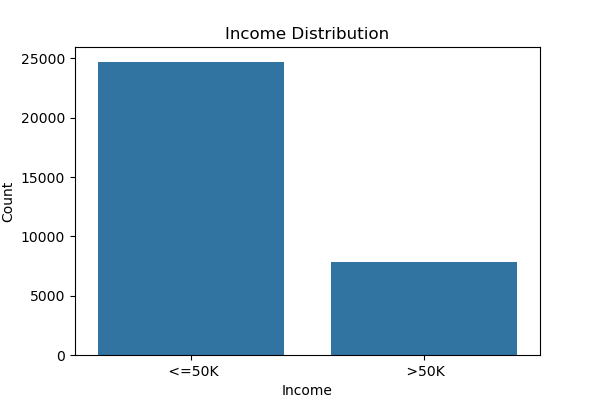
\includegraphics[width=0.5\linewidth]{1_IncomeDistribution.png}
  \caption{Income Distribution}
  \label{fig:income-distribution}
\end{figure}

% Figure 2: Age Distribution by Income
\begin{figure}[h]
  \centering
  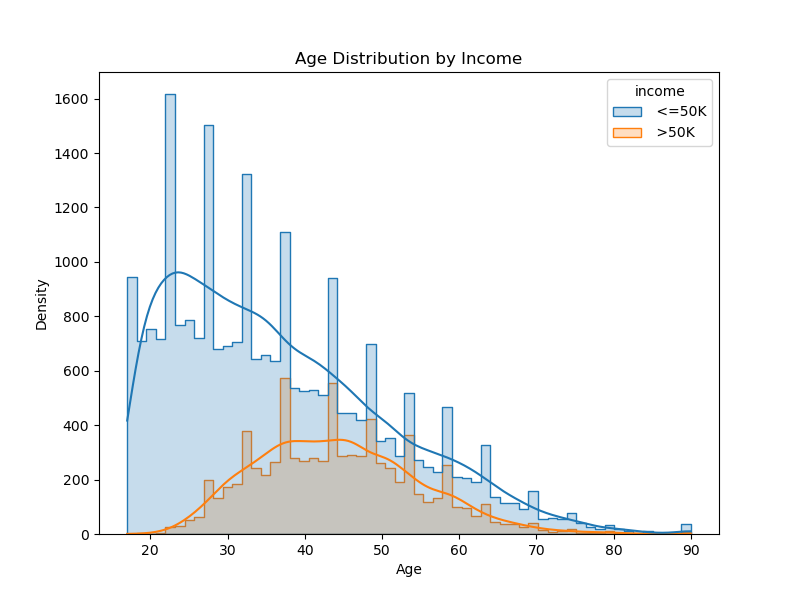
\includegraphics[width=0.5\linewidth]{2_AgeDistributionbyIncome.png}
  \caption{Age Distribution by Income}
  \label{fig:age-distribution-by-income}
\end{figure}

% Figure 3: Educations Levels by Income
\begin{figure}[h]
  \centering
  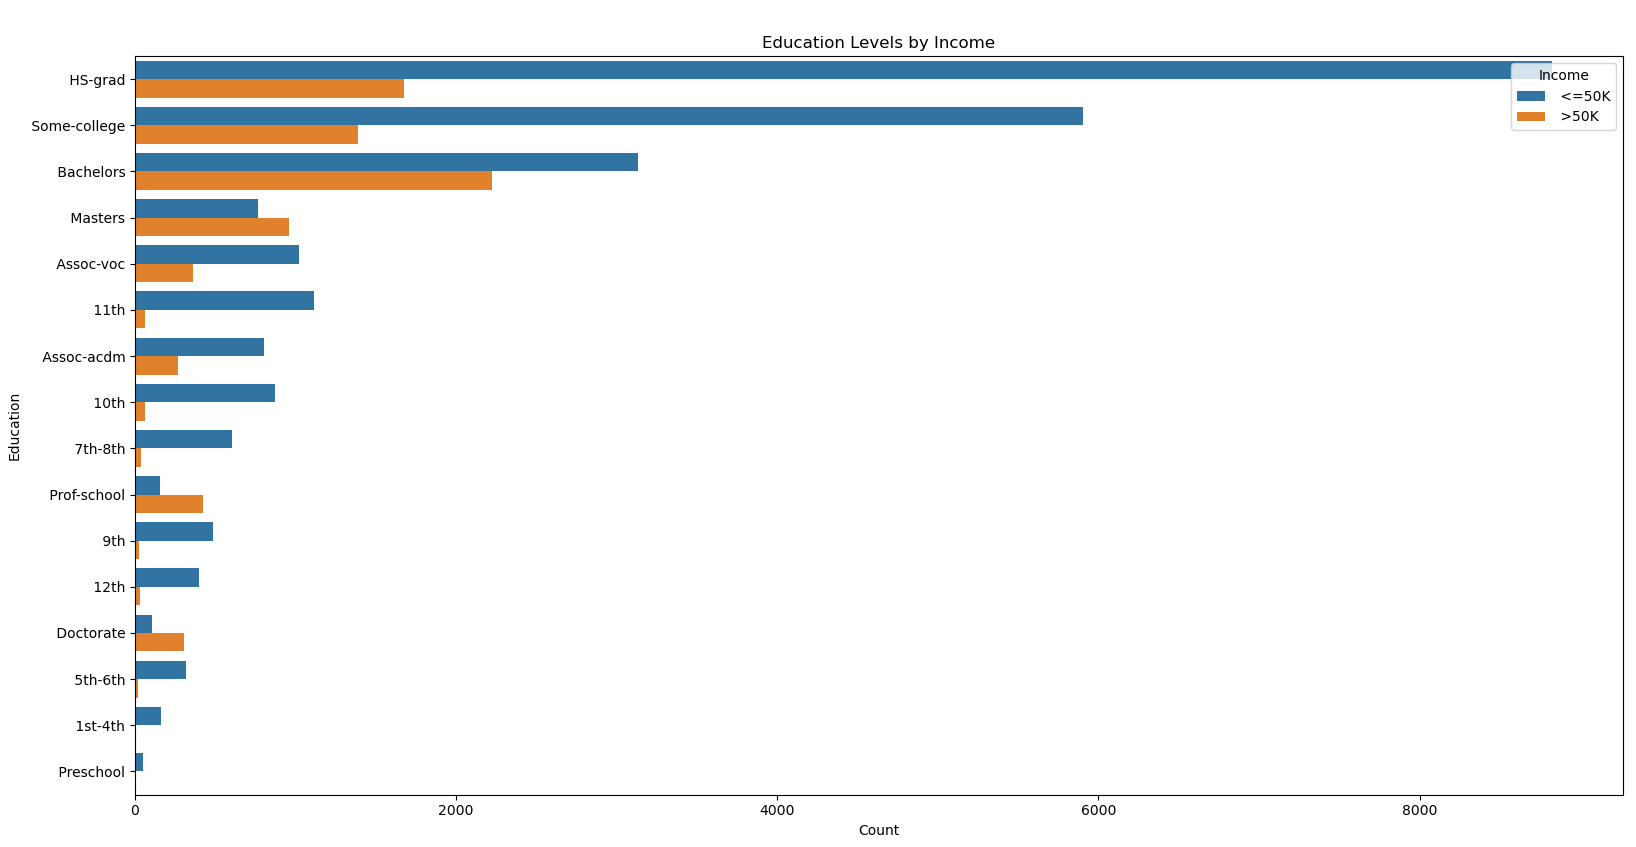
\includegraphics[width=0.5\linewidth]{3_EducationLevelsbyIncome.png}
  \caption{Education Levels by Income}
  \label{fig:education-levels-by-income}
\end{figure}

% Figure 4: Occupation vs Income
\begin{figure}[h]
  \centering
  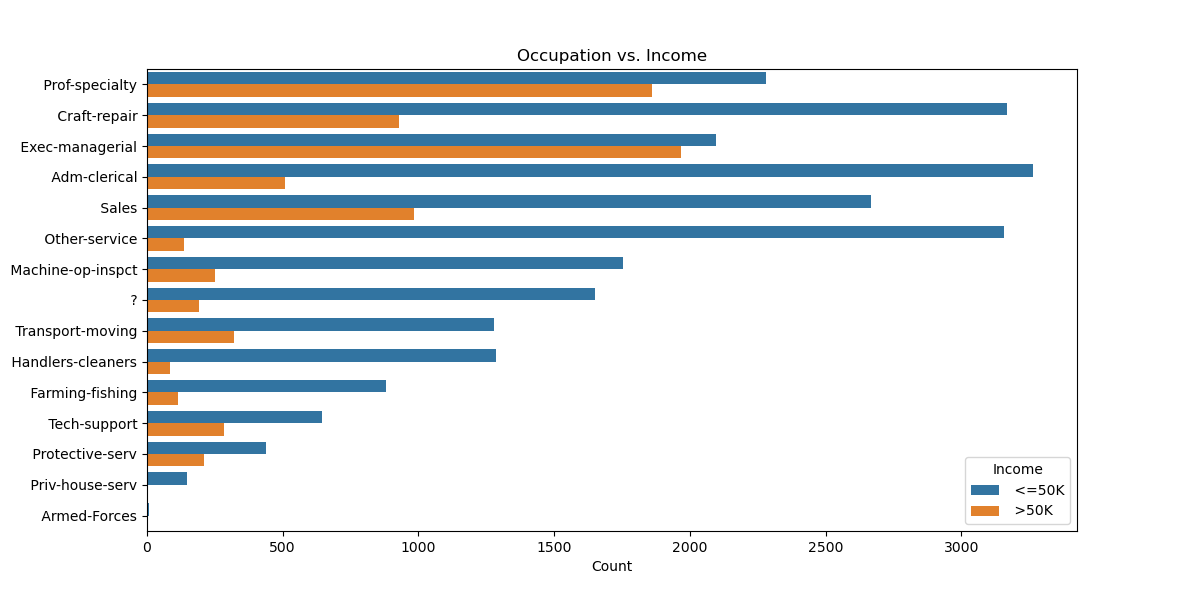
\includegraphics[width=0.5\linewidth]{4_OccupationvsIncome.png}
  \caption{Occupation vs. Income}
  \label{fig:occupation-vs-income}
\end{figure}

%there is no figure 5

\FloatBarrier  % This ensures Figure 5 appears immediately after Figure 4

% Figure 6: Age, Hours per Week, and Capital Gain vs. Income
\begin{figure}[h]
  \centering
  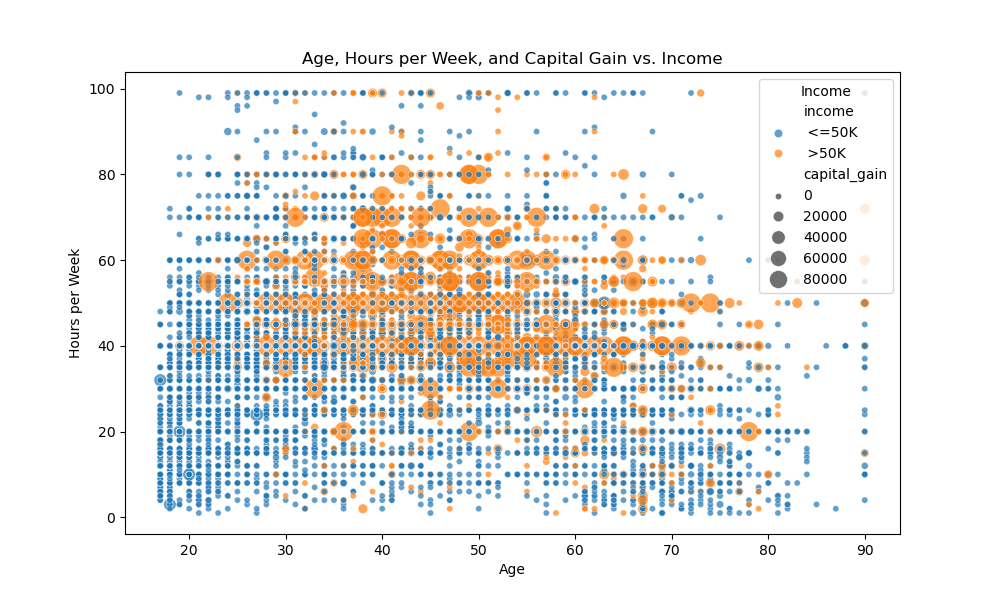
\includegraphics[width=0.5\linewidth]{6_AgeHoursperWeekandCapitalGainvsIncome.png}
  \caption{Age, Hours per Week, and Capital Gain vs. Income}
  \label{fig:age-hoursperweek-and-capitalgain-vs-income}
\end{figure}


\subsection{Figure 1: Income Distribution (Univariate Analysis)}
This figure helps to understand the overall distribution of income levels
that is crucial for determining income disparities. The dataset reveals that 
the majority of individuals earn $\leq$50K, highlighting an income imbalance.
This countplot was used to display categorical income distribution.
Since most individuals fall in the 50K category, marketing strategies
should focus on this group for career-advancement programs.

\subsection{Figure 2: Age Distribution (Univariate Analysis)}
This figure helped determine whether older individuals are more likely to 
earn $>$50K. While there was a slight increase in income with age, a 
significant number of older individuals still fall in the $\leq$50K category.
A histogram with KDE (Kernel Density Estimate) was used to visualize the 
age distribution by income. Age alone is not a strong predictor of income; 
other factors such as education and occupation have a greater impact.

\subsection{Figure 3: Education Levels by Inncome (Bivariate Analysis)}
Higher education is often linked to better job opportunities and higher 
income levels. Individuals with higher education levels (Masters, Doctorate, 
and Bachelors) have a significantly higher probability of earning $>$50K. 
A countplot was used to compare education levels against income categories. 
Marketing efforts should be directed towards bachelor's degree holders 
looking to upskill, as they represent a key segment likely to enroll in 
educational programs.

\subsection{Figure 4: Occupation vs. Income (Bivariate Analysis)}
To analyze which occupations have the highest proportion of high earners. 
Executive, managerial, and professional roles show a higher proportion of 
individuals earning $>$50K, whereas service-oriented jobs have lower income 
levels. A countplot was used to analyze occupation-based income distribution. 
High-income occupations could be targeted for specialized executive education 
programs.

\subsection{Figure 5: Age, Hours per Week, and Capital Gain vs. Income (Multivariate Analysis)}
To analyze how multiple factors interact to impact income. Higher-income 
individuals tend to work more hours and have higher capital gains, but age 
alone is not a strong predictor. A scatterplot with hue and size variations 
was used to visualize trends. Capital gain has a significant impact on income, 
but work hours alone do not guarantee higher earnings. This suggests that 
financial investments may play a role in distinguishing high earners.


\section{Questions}
During the course of the analysis, several challenges were encountered:
\subsubsection{Missing Values}Approximately 1,800 rows contained missing values 
in attributes such as workclass, occupation, and native-country. Handling 
missing values was crucial for ensuring data quality. Since these missing 
values were distributed across multiple variables, careful consideration was 
required to decide whether to impute or remove them. Removing these rows 
ensured that the analysis remained unbiased but also resulted in the loss 
of some data.
\subsubsection{Income Imbalance}The dataset had a significant skew, with about 
76\% of individuals earning $\leq$50K. This imbalance made it difficult to 
draw equally weighted insights across income categories. Visualizations 
required careful interpretation, and statistical normalization techniques 
were considered but not implemented in this phase of the project.
\subsubsection{Correlations Between Attributes}Some attributes, such as 
education, showed a strong relationship with income, while others, such as 
hours worked per week, presented a more complex pattern. The challenge was to 
determine which attributes had the highest predictive power for income level 
and how these attributes interacted in multivariate relationships. This 
required exploratory data analysis techniques such as scatter plots and 
correlation heatmaps.

\section{Solutions}
To address the challenges that were faced, the following solutions were implemented:
\subsubsection{Data Cleaning}Rows with missing values were removed to 
prevent bias and ensure accurate analysis. While imputation techniques 
such as mean substitution were considered, it was decided that removing 
missing values would maintain the dataset's integrity without introducing 
artificial patterns.
\subsubsection{Normalized of Data}Rows with missing values were removed to 
prevent bias and ensure accurate analysis. While imputation techniques 
such as mean substitution were considered, it was decided that removing 
missing values would maintain the dataset's integrity without introducing 
artificial patterns.
\subsubsection{Multivariate Analysis}To handle complex relationships 
between attributes, scatter plots and pair plots were used to visually 
inspect correlations. These analyses helped confirm that education and 
occupation were the strongest determinants of income. Additionally, multivariate
 plots were used to explore the interaction of age, hours worked, and capital 
 gains to ensure a thorough understanding of their influence on income.
\subsubsection{Feature Engineering Considerations}Although not implemented 
in this phase, potential strategies such as creating new categorical bins 
for age groups or aggregating occupations into broader categories were explored 
for future analysis.

\section{Not Doing for Future Work}
\subsubsection{Predtictive Modeling}A supervised machine learning model 
(e.g., logistic regression, decision trees, or neural networks) could be 
developed to predict income levels based on demographic attributes. This 
would allow for a more precise assessment of income determinants and 
could be used to develop targeted marketing strategies for UVW College.
\subsubsection{Geographic Segmentation}The dataset includes a variable 
for native country, which was not extensively analyzed in this report. 
Future research could explore how income levels vary across different 
geographic locations and whether certain countries have a stronger 
correlation with high-income individuals.
\subsubsection{Expanded Feature Engineering}New features could be derived, 
such as aggregating education levels into fewer categories (e.g., High 
School, Bachelor’s, Advanced Degree) or creating new interaction terms 
between key variables like work hours and education. These features could 
improve the robustness of future models.
\subsubsection{Incorporating External Socioeconomic Data}Future work could 
involve merging the dataset with additional economic indicators, such as 
unemployment rates, inflation, or industry growth statistics. This would 
provide a more comprehensive understanding of how macroeconomic factors 
influence income levels.


By implementing these enhancements, future studies can provide even deeper 
insights into income distribution and help UVW College refine its approach 
to targeting students based on financial stability and career progression.


\section{Conclusion}
The analysis of the UCI Adult dataset has provided significant insights into the 
factors influencing income levels. Education and occupation emerged as the strongest 
determinants of income, whereas factors like age and work hours showed 
limited predictive power. The findings suggest that higher education and 
professional roles correlate with greater financial success, reinforcing the 
importance of academic and career advancement programs.

For UVW College, these insights can drive targeted marketing efforts toward 
individuals seeking career growth and skill enhancement. Given the strong influence 
of education on income, programs designed for upskilling and executive education 
should be prioritized. Additionally, capital gains were found to be a critical 
differentiator among high-income earners, indicating that financial literacy and 
investment-oriented education could also be valuable offerings.

Future studies could incorporate predictive modeling techniques and external 
socio-economic data to enhance the analysis. Expanding the dataset to include 
geographic and industry-specific variables would further refine the understanding 
of income distribution trends. By continuously leveraging data-driven insights, UVW 
College can develop strategies to effectively engage its target audience and support 
their professional aspirations.
% use section* for acknowledgment
\section*{Acknowledgment}


The author would like to thank Professor Ghayekhloo and the Teaching Assistants for instructing this course and providing the resources to complete this course's final project.


% that's all folks
\end{document}
